\section{Mathematik}
\subsection{Mathematical Analysis for Science and Technology Majors}
This course is all about calculus, both single variable and multi variate. I've learnt limit, differential, integral, differential equation, and series.

\subsection{Linear Algebra and Analytic Geometry}
This course covers Matrix theory, eigenvalues and eigenvectors and vector spaces.

\subsection{Probability Theory and Mathematical Statistics}
This course talks about Discrete probability distributions(Poisson distribution, the Bernoulli distribution, the binomial distribution, the geometric distribution), Continuous probability distributions(Normal distribution), Law of large numbers and Central limit theorem.

\subsection{Computational methods}
This course introduces the basis of numerical method, including integration(Simpson's rule), differential equation(Runge Kutta methods), interpolation(Newton polynomial), curve fitting(least square).

\subsection{Complex Function and Integral Transformation}
This course talks about the basic of Complex analysis, as well as Fourier Transform and Laplace Transform.

\subsection{Signals and Systems I}
This course covers the basic theory of LTI systems and mathematical modeling of signal and systems. Because LTI Systems are the easiest systems to work with, and they are ideal to analyze and design. It investigates the response of a linear and time-invariant system to an arbitrary input signal. The purpose of the course is that it provides a tool to analysis a system(circuit system, for example), and introduces the concept of (complex) frequency domain.

\subsubsection{Signals}
 ``A signal is a function of independent variables that carry some information."

There are numerous types of signal, but can be categorized as continuous signals and discrete signals. One of the most important class of signals are sinusoidal signals. Because any periodic signal can be decomposed to linear combination of a set of sinusoid signals.

\paragraph{Typical Signals}
\begin{itemize}
  \item Unit Impulse function
  $$u(t)$$
  \item Unit Step function
  $$\delta(t)$$
  \item Sa function
  $$\frac{\textrm{sin}(\pi t)}{t}$$
\end{itemize}

\paragraph{What is the difference between power signal and energy signal?}
\begin{enumerate}
  \item Energy signals are time limited while power signals can exist over infinite time.
  \item Non periodic signals are energy signals while power signals are periodic.
  \item Power of an energy signal is zero and the energy of a power signals is infinite.
\end{enumerate}
But an energy signal has zero power, because energy is power integrated over all time. When you find the power in an energy signal, you have a finite energy divided by infinity. Thus zero.

\subparagraph{Parseval’s equation}
$$\int_{-\infty}^{\infty}|x(t)|^2dt=\int_{-\infty}^{\infty}|X(f)|^2df$$

\subparagraph{Power Spectrum}
$$P=\lim_{T\to \infty}\frac{1}{2T}\int_{-T}^{T}x^2(t)dt$$

\paragraph{Gibbs phenomenon}
The Gibbs phenomenon involves both the fact that Fourier sums overshoot at a jump discontinuity, and that this overshoot does not die out as the frequency increases.

\subsubsection{Systems}

\paragraph{LTI System} Ein System heißt linear, wenn die beiden folgenden Bedingungen erfüllt sind:

\begin{itemize}
  \item Verstärkungsprinzip: $f(k\cdot u(t))=k\cdot f(u(t))$
  \item Überlagerungsprinzip: $f\left(u_1\left(t\right)\right)+f\left(u_2\left(t\right)\right) =
f\left(u_1\left(t\right)+u_2\left(t\right)\right)$
\end{itemize}

Wenn eine oder beide dieser Bedingungen nicht erfüllt sind, heißt das System nichtlinear.

\subparagraph{Time Invariance} If the input signal $x(t)$ produces an output $y(t)$ then any time shifted input, $x(t + \delta)$, results in a time-shifted output $y(t + \delta)$.

\subparagraph{Memory} A system is said to have memory if the output from the system is dependent on past inputs (or future inputs) to the system.

\subparagraph{Causality} Causality is a property that is very similar to memory. A system is called \textbf{causal} if it is only dependent on past or current inputs.

\subparagraph{BIBO Stability} For instance, if we apply 5 volts to the input terminals of a given circuit, we would like it if the circuit output didn't approach infinity, and the circuit itself didn't melt or explode. This type of stability is often known as "Bounded Input, Bounded Output" stability, or BIBO.

\paragraph{Warum LTI System?}

Viele technische Systeme wie in der Nachrichten- oder Regelungstechnik weisen, zumindest in guter N\"aherung, diese Eigenschaften auf.

\subparagraph{Responses}
\begin{itemize}
  \item Zero-State Response $\leftrightarrow$ Zero-Input Response
  \item Transitional Response $\leftrightarrow$ Steady-State Response
  \item Frequency Response

  The frequency response of a system is defined as the steady-state response of the system to a sinusoidal signal.
\end{itemize}

\subparagraph{Natural Frequency} Natural frequency is the frequency at which a system tends to oscillate in the absence of any driving or damping force. Natural frequencies depend only on network topology and element values but not the input. All poles of the network transfer function are also natural frequencies of the corresponding response variable, however there may exist some natural frequencies that are not a pole of the network function, these frequencies happen at some special initial states.

\subsubsection{Sampling Theorem}
Sampling is the process of converting a signal (for example, a function of continuous time and/or space) into a numeric sequence (a function of discrete time and/or space).

If a function x(t) contains no frequencies higher than B hertz, a sufficient sample-rate is therefore 2B samples/second, or anything larger. Equivalently, for a given sample rate fs, perfect reconstruction is guaranteed possible for a bandlimit $B \leq fs/2$.

\subsubsection{What is group delay?}
Group delay is:
The basic idea of group delay is reasonably simple; the negative derivative of phase with respect to frequency. Since it is a derivative, if the phase is linear, the group delay is a constant.
\begin{enumerate}
  \item A measure of device phase distortion.
  \item The transit time of a signal through a device versus frequency.
  \item The derivative of the device's phase characteristic with respect to frequency.
\end{enumerate}

In Time domain: $r(t)=ke(t-t_0)$

And for frequency domain: $R(j\omega)=kE(j\omega)e^{-j\omega t_0}$

the transfer function is: $H(j\omega)=\frac{R(j\omega)}{E(j\omega)}=ke^{-j\omega t_0}$

Thus $\varphi(\omega)=-\omega t_0$.

So, in a way, the group delay is giving you information about how the sidebands will be delayed relative to that carrier frequency, and applying that delay will change the shape of the amplitude envelope in some way.

%\includepdfmerge{includes/lti2.pdf, 1-15}

\subsection{Principles of Automatic Control II}
This course mainly talks about the concept of control system, feedback, and stability. I've learnt from the course that how to analysis and design a control system, both in time domain and frequency domain.

There are two types of automatic control system for different purposes:
\begin{itemize}
  \item Regulator: keep output at a steady, known value
  \item Servo system: Make output track a reference system
\end{itemize}

\subsubsection{Open Loop vs Closed Loop Control}

\begin{figure}
  \centering
  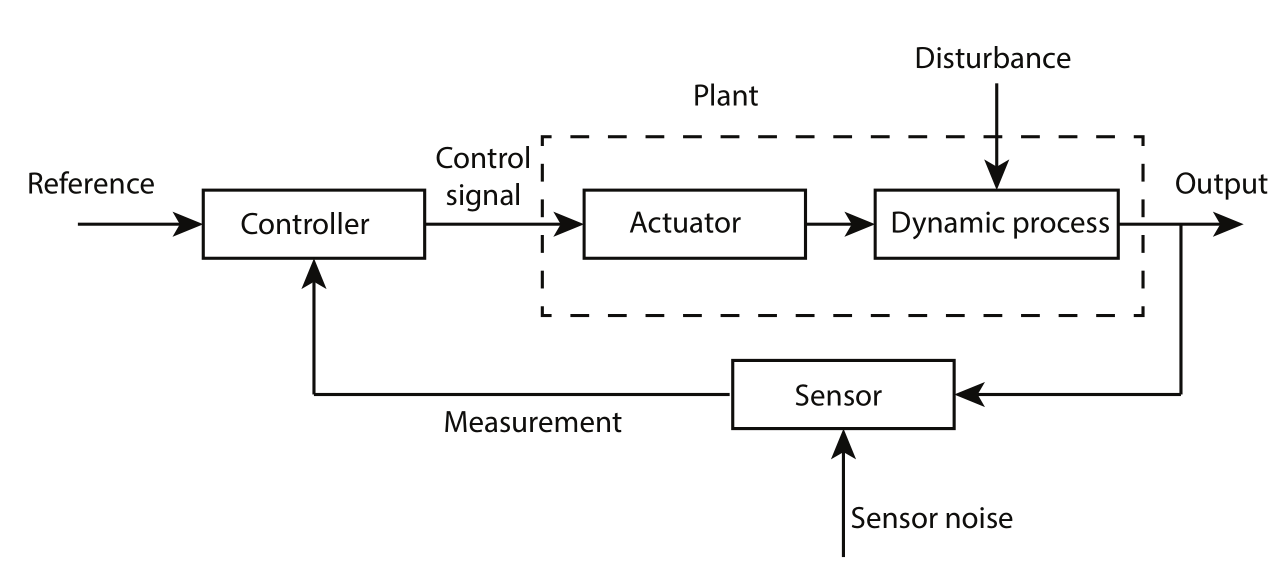
\includegraphics[width=4in]{fig/800px-Feedback_loop_with_descriptions.svg.png}
  \caption{A typical control system}\label{fig_control_loop}
\end{figure}

A closed-loop system uses a measurement of the output signal and a comparison with the desired output to generate an error signal that is used by the controller to adjust the actuator. One of the key concept in the principle of automatic control lies in feedback control.

Despite the cost and increased system complexity, closed-loop feedback control has the following advantages:
\begin{itemize}
  \item Decreased sensitivity of the system to variations in the parameters of the process
  \item Improved rejection of the disturbances.
  \item Improved reduction of the steady-state error of the system.
\end{itemize}

\begin{figure}
  \centering
  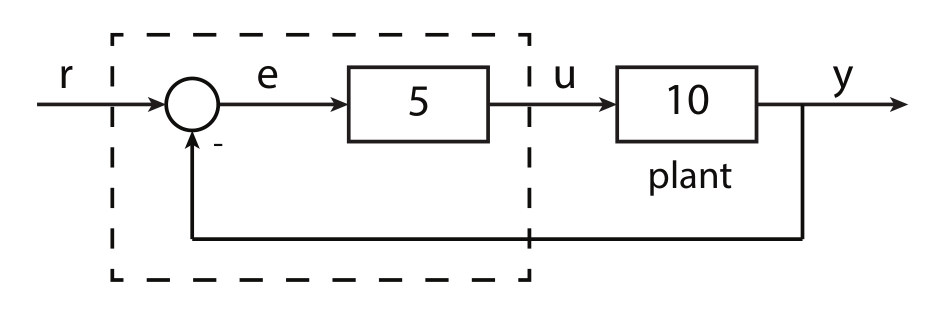
\includegraphics[width=1.8in]{fig/fig_control_example.png}
  \caption{A closed loop control system}\label{fig_control_system}
\end{figure}


\paragraph{Example} A control system is shown as figure \ref{fig_control_system}.

Look at transfer functions from r to y:

\begin{center}
    \begin{tabular}{c|c|c}
      %\hline
      % after \\: \hline or \cline{col1-col2} \cline{col3-col4} ...
        & Open Loop & Closed Loop \\
        \hline
      $\frac{y}{r}$ & $\frac{1}{10} \cdot 10 = 1$ & $\frac{5 \cdot 10}{1+5 \cdot 10} = \frac{50}{51} \approx 0.98$ \\
      %\hline
    \end{tabular}
\end{center}

We want $\frac{y}{r}=1$, so at first glance, it looks like open-loop is better than closed-loop. However, consider what happens if it turns out our plant model was wrong(or changes), so that really G=15. Then

\begin{center}
    \begin{tabular}{c|c|c}
      %\hline
      % after \\: \hline or \cline{col1-col2} \cline{col3-col4} ...
        & Open Loop & Closed Loop \\
        \hline
      $\frac{y}{r}$ & $\frac{1}{10} \cdot 15 = 1.5$ & $\frac{5 \cdot 15}{1+5 \cdot 15} = \frac{75}{76} \approx 0.9868$ \\
      %\hline
    \end{tabular}
\end{center}

That is, if the plant gain changes by 50\%, the transfer function of the open-loop system will vary by -5\%. However, the transfer function of the closed-loop system will vary by only 0.66\% (in this case).

\subparagraph{Big Idea} High gain control loop reduces the sensitivity of
the control system to variations in the plant.

\subsubsection{Time Domain Specifications}
Given a 2nd order system transfer function:
$$H(s)=\frac{\omega ^2 _n}{s^2+2\zeta \omega _n s + \omega ^2 _n} $$

Typical response is shown in figure \ref{fig_step_response}.
\begin{figure}
  \centering
  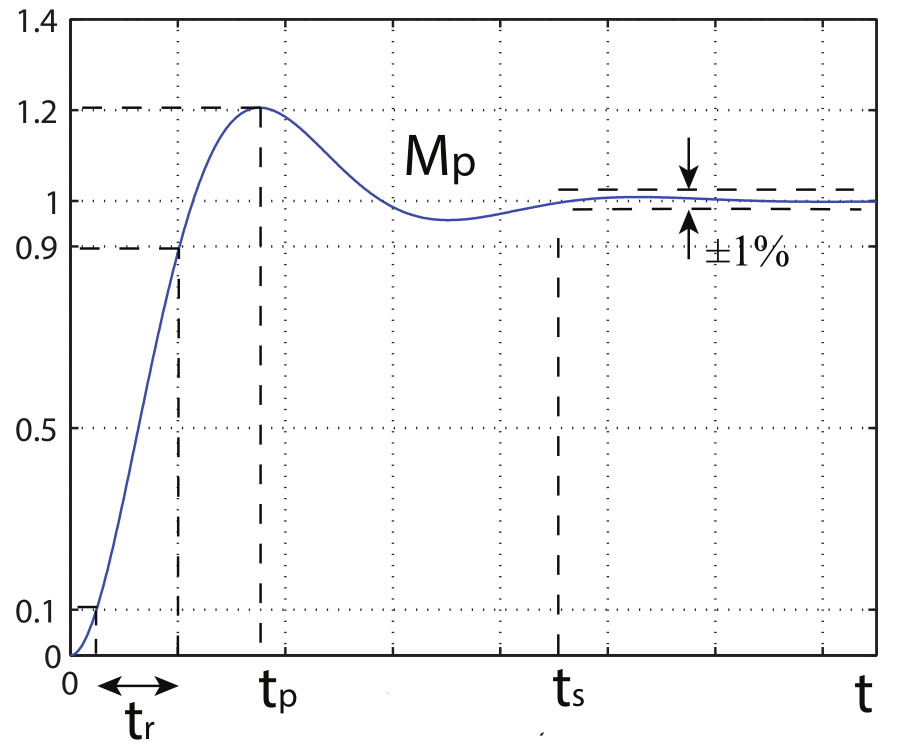
\includegraphics[width=2.5in]{fig/cntr_step.png}
  \caption{step response of a 2nd order system}\label{fig_step_response}
\end{figure}

$M_p$ = peak overshoot

$t_r$ = rise time (10\% to 90\%)

$t_s$ = settling time (1\%)

$t_p$ = time of peak

The step response of H(s) is:
$$h_s(t)=1-e^{-\zeta \omega _n t}(\textrm{cos}(\omega _d t) + \frac{1}{\sqrt{1-\zeta ^2 }}\textrm{sin}(\omega _d t))$$

\subsubsection{Übertragungsfunktion}
Die Übertragungsfunktion oder auch Systemfunktion beschreibt in der ingenieurwissenschaftlichen Systemtheorie mathematisch die Beziehung zwischen dem Ein- und Ausgangssignal eines dynamischen Systems im Frequenzraum.

$$G(s) = \frac{Y(s)}{U(s)} = \frac{\mathcal L \{ y(t) \} }{\mathcal L\{ u(t) \} }$$

%\subsubsection{Second Order System}
%
%$$\Phi(s)= \frac{1}{T^2s^2+2\zeta Ts+1}=\frac{\omega^2_n}{s^2+2\zeta \omega_n s+\omega^2_n}$$
%
%$\omega_n$ is natural frequency, and $\zeta$ is damping ratio.

\subsubsection{Stability}
Stability of closed-loop feedback systems is central to control system design. A stable system should exhibit a bounded output if the corresponding input is bounded (BIBO stable).

\paragraph{The Routh Stability Criterion} The closed-loop system is stable if $$\Re(p_i)<0, \forall i$$

Can we tell if the system is stable, without actually solving for the roots?

For \emph{Routth Array}, if all of its coefficient is positive, then the system$$a_ns^n+a_{n-1}s^{n-1}+\dots+a_1s+a_0=0$$is stable.


\begin{tabular}{ccccc}
  %\hline
  % after \\: \hline or \cline{col1-col2} \cline{col3-col4} ...
  Row n: & $a_n$ & $a_{n-2}$ & $a_{n-4}$ & $\dots$ \\
  Row n-1: & $a_{n-1}$ & $a_{n-3}$ & $a_{n-5}$ & $\dots$ \\
  Row n-2: & $b_1$ & $b_2$ & $b_3$ & $\dots$ \\
  Row n-3: & $c_1$ & $c_2$ & $c_3$ & $\dots$ \\
  $\vdots$ &   & $\ddots$ &   &   \\
  Row 3: & * & * &  &\\
  Row 2: & * &   &   &   \\
  Row 1: & * &   &   &   \\
  %\hline
\end{tabular}

The number of unstable poles is the number of sign changes in the first column of the array.

\paragraph{Wurzelortskurve}

$$G_0(s) = k \hat{G}_0(s) = k \frac{\Pi_{i=1}^{q}(s-s_{0i})}{\Pi_{i=1}^{n}(s-s_i)}$$

\begin{enumerate}
  \item Ursprung/Ende: Jeder Ast der Wurzelortskurve beginnt in einem Pol der offenen Kette $G_0$ und endet in einer Nullstelle der offenen Kette, oder im Unendlichen.
  \item Asymptoten: Für große Verstärkungen nähern sich die Äste Geraden asymptotisch an. Die Anzahl der Asymptoten ist $n-q$. Die Asymptoten haben für $k>0$ Neigungswinkel $\phi_\mathrm{As} = \frac{\pi+ l \cdot 2 \pi}{n-q}, \quad l=0,1,...,n-q-1$ und schneiden sich im gemeinsamen Schnittpunkt (Wurzelschwerpunkt) $s_\mathrm{As} = \frac{\sum_{i=1}^{n}s_i-\sum_{i=1}^{q}s_{0i}}{n-q}$.
  \item Reelle Achse: Zur eigentlichen Wurzelortskurve gehören genau die Punkte $s$ der reellen Achse, für die die Anzahl der von dort aus gesehen rechts gelegenen reellen kritischen Stellen (Nullstellen und Pole) ungerade ist. Alle übrigen Punkte auf der reellen Achse gehören zur komplementären WOK ($k<0$). Jeder Punkt auf der reellen Achse ist also Teil einer WOK: entweder Teil der eigentlichen WOK ($k>0$) oder Teil der komplementären WOK ($k<0$).
  \item Verzweigungs- und Vereinigungspunkte: Verzweigungs- und Vereinigungspunkte sind genau solche Punkte, die sowohl die Phasenbedingung als auch die Gleichung $\sum_{i=1}^{q} \frac{1}{s-s_{0i}} = \sum_{i=1}^{n}\frac{1}{s-s_i}$ erfüllen.
\end{enumerate}


\paragraph{Frequency Criteria} If the gain for frequencies which have phase delay over $-180^\circ$ is greater than 1, then the system has positive feedback loop for those frequencies, which may cause the system unstable.

\subparagraph{Bode-Diagramm} Ein Bode-Diagramm beschreibt den Zusammenhang zwischen einer harmonischen Anregung („schwingung“) an einem Eingang des Systems und dem zugehörigen Ausgangssignal im stationären Zustand, d.h. für t→∞.

\subsubsection{PID controller}
\begin{itemize}
  \item Increase \textbf{P (proportional)} would speed up the system response, but decrease system damping.
  \item Increase \textbf{I (integral)} would reduce system steady-state error, but may cause overshoot.
  \item Increase \textbf{D (derivative)} would increase system damping, but is affected by noise.
\end{itemize}

\subsubsection{Compensation}
Compensation is the use of a dynamic controller $K(s)$ (as opposed to proportional control) to improve the system's stability and error characteristic.

\paragraph{Lead Compensation}

When the phase margin doesn't meet the stability requirement, then Lead Compensation may be deployed to acquire lower phase lag. One problem with PD controller is that the gain gets large at high frequencies. So instead use lead compensator:

$$G_c(s)=\frac{1+\alpha Ts}{1+Ts}, \alpha >1$$

\begin{figure}
  \centering
  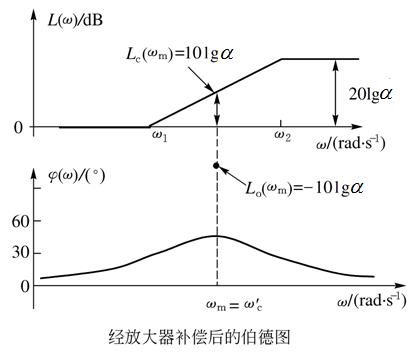
\includegraphics[width=2.4in]{fig/Lead_Compensation.png}
  \caption{Bode Diagram of Lead Compensation}\label{fig_lead}
\end{figure}


\paragraph{Lag Compensation}

In the situation where stable gain is expected to be enlarged, with little influence on dynamic gain, then Lag Compensation is the choice.

$$G_c(s)=\frac{\beta Ts+1}{Ts+1}$$

\begin{figure}
  \centering
  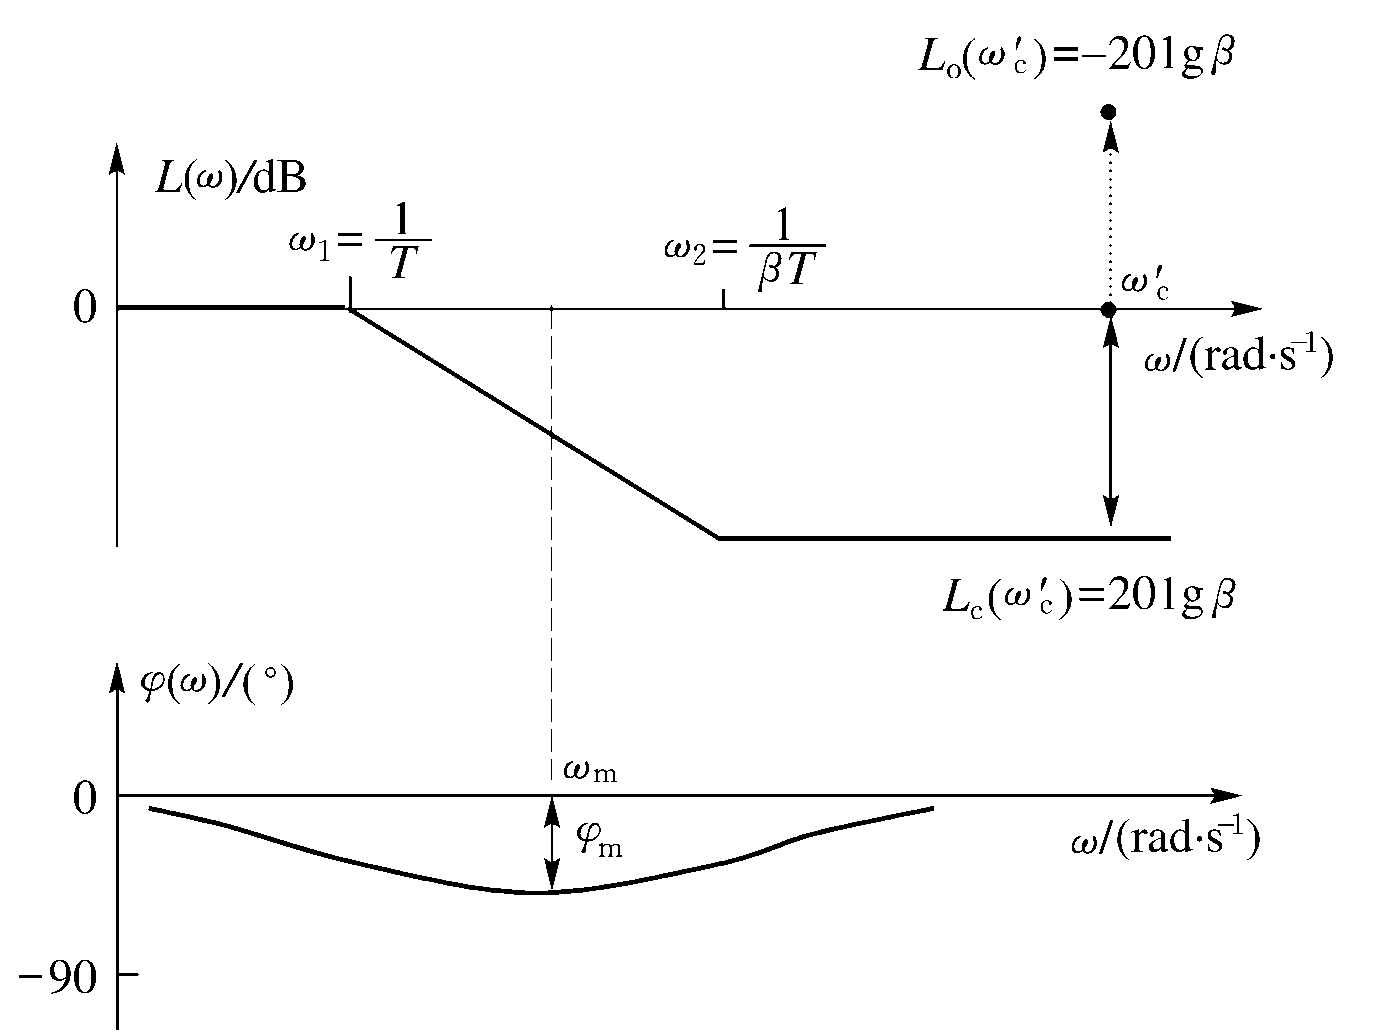
\includegraphics[width=3.5in]{fig/Lag_Compensation.png}
  \caption{Bode Diagram of Lag Compensation}\label{fig_lag}
\end{figure}


%\textbf{We look primarily at four types of compensation:}
%
%$
%\left.
%\begin{aligned}
%  \textrm{PD Control} \\
%  \textrm{Lead Compensation}
%\end{aligned}
%\right\}
%$ used primarily to add lead at the crossover frequency,
% allowing the compensated system to have a faster speed of response and/or have more damping.
%
%$
%\left.
%\begin{aligned}
%  \textrm{PI Control} \\
%  \textrm{Lag Compensation}
%\end{aligned}
%\right\}
%$ used primarily to increase the frequency response magnitude at low frequencies, reducing steady-state tracking errors.

\subsubsection{State Space(Zustandsraumdarstellung)}
The state-space representation (also known as the ``time-domain approach'') provides a convenient and compact way to model and analyze systems with multiple inputs and outputs.

\begin{figure}
  \centering
  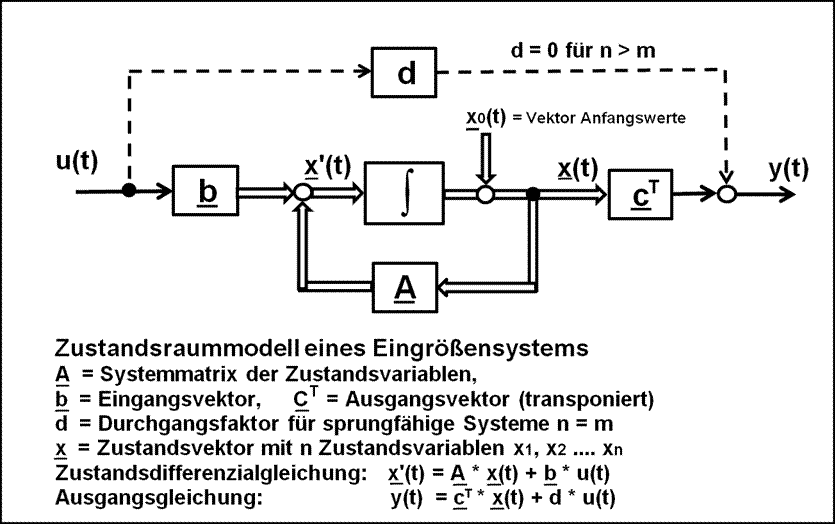
\includegraphics[width=4.5in]{fig/Zustandsraummodell_eines_eingroessensystems.png}
  \caption{Symbolisches Blockschaltbild eines Modells eines Übertragungssystems in der Zustandsraumdarstellung für ein Eingrößensystem.}\label{fig_Zustandraumdarstellung}
\end{figure}

\paragraph{State} The internal state variables are the smallest possible subset of system variables that can represent the entire state of the system at any given time.

\paragraph{Controllability} State controllability condition implies that it is possible – by admissible inputs – to steer the states from any initial value to any final value within some finite time window.  Au\ss erdem, Ausgangssignale des Systems gilt als Steuerbarkeit auch.
%A continuous time-invariant linear state-space model is controllable if and only if
%\begin{equation*}
%  \textrm{rank}
%  \begin{bmatrix}
%    B & AB & A^2B & \dots & A^{n-1}B
%  \end{bmatrix}=n
%\end{equation*}

\paragraph{Observability} Observability is a measure for how well internal states of a system can be inferred by knowledge of its external outputs.
%A continuous time-invariant linear state-space model is observable if and only if
%\begin{equation*}
%  \textrm{rank}
%  \begin{bmatrix}
%    C \\
%    CA \\
%    \vdots \\
%    CA^{n-1}
%  \end{bmatrix}=n
%\end{equation*}

%\includepdfmerge{includes/control_glossar.pdf, 1-12}

\paragraph{Beobachter}

Häufig können aus technischen oder kommerziellen Gründen nicht alle Zustandsvariablen gemessen werden. Deshalb werden einzelne nicht messbare Zustandsvariablen aus den bekannten und vorhandenen Eingangs- und Ausgangsgrößen der Regelstrecke errechnet. Zustandsbeobachter, die diese Aufgabe durchführen, sind zusätzliche Regelsysteme. Sie rekonstruieren Zustandsvariable aus dem Verlauf der Ein- und Ausgangsgrößen an einem Modell der Regelstrecke.

\subsection{Digital Signal Processing(Bilingual)}
This course, to be more specific, talks about how to analyze discrete time signals. I've learnt from this course, how to handle discrete time signal, the FFT Algorithm, how to design a digital filter(IIR and FIR).

\subsubsection{Objekt: Was ist ein Signal?}

Ein digitales Signal ist, im Gegensatz zu den kontinuierlichen Funktionen der analogen Signalverarbeitung, diskret in Zeit- und Wertebereich, also eine Folge von Elementarsignalen (z. B. Rechteckimpulsen). Diese Folge entsteht meist in einem zeit- oder ortsperiodischen Messprozess. So wird zum Beispiel Schall über die Auslenkung einer Membran oder Verbiegung eines Piezokristalls in eine elektrische Spannung umgewandelt und diese Spannung mittels eines AD-Wandlers zeitperiodisch wiederholt in digitale Daten konvertiert. Solch ein realistischer Messprozess ist endlich, die entstehende Folge besitzt einen Anfangsindex $\alpha$ und einen Endindex $\omega$.

\begin{figure}
  \centering
  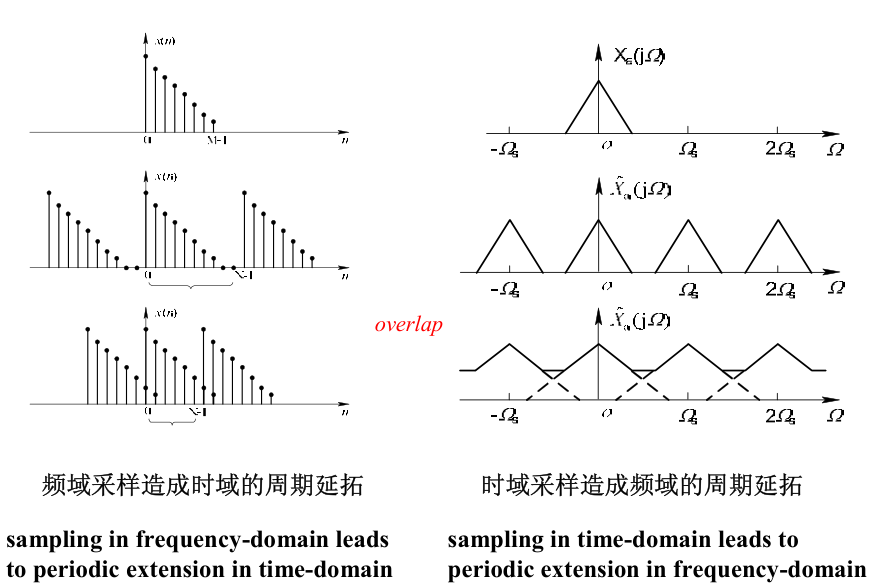
\includegraphics[width=4.2in]{fig/dsp_relationship.png}
  \caption{Relationship between time domain and frequency domain sampling}\label{fig_dsp_sampling}
\end{figure}

\subsubsection{DFT}
A periodic sequence $\tilde{x}(n)=\tilde{x}(n+rN), r\in Z$ can be represented by a Fourier series $\tilde{x}(n)=\displaystyle{\sum_{k=0}^{N-1}a_ke^{j\frac{2\pi}{N}kn}}$, where
$$a_k = \frac{1}{N}\displaystyle{\sum_{n=0}^{N-1}\tilde{x}(n)e^{-j\frac{2\pi}{N}kn}}$$

and thus
$$\tilde{X}(k)=Na_k=DFS[\tilde{x}(n)]=\displaystyle{\sum_{n=0}^{N-1}\tilde{x}(n)e^{-j\frac{2\pi}{N}kn}}$$
$$\tilde{x}(n)=IDFS[\tilde{X}(k)]=\frac{1}{N}\displaystyle{\sum_{k=0}^{N-1}\tilde{X}(k)e^{j\frac{2\pi}{N}kn}}$$

Relationship between time domain and frequency domain:
\begin{itemize}
  \item continuous $\leftrightarrow$ nonperiodic
  \item discrete $\leftrightarrow$ periodic
\end{itemize}

\subsubsection{DIT-FFT}
It re-expresses the DFT of an arbitrary composite size $N = N_1N_2$ in terms of smaller DFTs of sizes $N_1$ and $N_2$, recursively, to reduce the computation time to $O(N log N)$.

Separate x(n) into two (N/2)-point sequences consisting of the even-numbered points and odd-numbered points.
$$
\left\{
    \begin{aligned}
      x_1(r) &= x(2r) \\
      x_2(r) &= x(2r+1)
    \end{aligned}
\right.
$$

And then perform Butterfly Computation

$$
\left\{
    \begin{aligned}
      X(k) &= X_1(k)+W_n^kX_2(k) \\
      X(k+\frac{N}{2}) &= X_1(k)-W_n^kX_2(k)
    \end{aligned}
\right.
$$

\begin{figure}
  \centering
  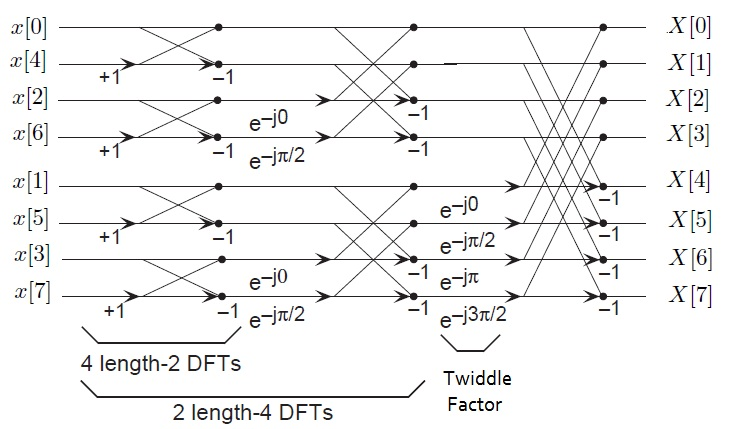
\includegraphics[width=3.5in]{fig/FFt.jpg}
  \caption{Data flow diagram for N=8}\label{fig_fft}
\end{figure}

\subsubsection{IIR Filter}

An IIR Filter of order N the transfer function:

\begin{align*}
H(z) & = \frac{\sum_{i=0}^P b_{i} z^{-i}}{1+\sum_{j=1}^Q a_{j} z^{-j}}
\end{align*}

IIR filters have much better frequency response than FIR filters of the same order. Unlike FIR filters, their phase characteristic is not linear which can cause a problem to the systems which need phase linearity.

\paragraph{Design Flow}

Die Aufgabe des Filterentwurfs ist es, eine rationale Funktion von $z^{-1}$ zu finden, die das Toleranzschema auf dem Einheiskreis $z=e^{j\Omega}$ erf\"ullt.

\begin{figure}
  \centering
  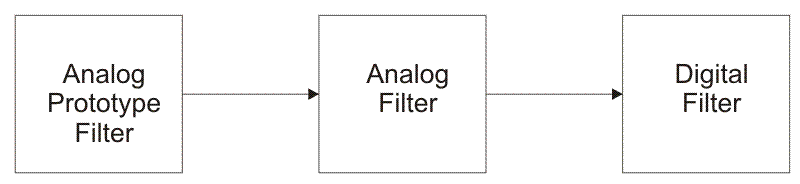
\includegraphics[width=2.5in]{fig/fig3-1-2.png}
  \caption{Block diagram of design method using reference analog prototype filter}\label{fig_iir}
\end{figure}

First step is design analog low-pass filter, whose parameter is selected base on the desired characteristic of IIR filter. The second step is to convert the low-pass one to the desired pass band.

The last step is perform either Transformation via Impulse Invariance ($z_i=e^{s_iT}$, $\omega = \Omega T$), or Bilinear Transformation ($s=\frac{2}{T}\frac{1-z^{-1}}{1+z^{-1}}$, $\Omega = \frac{2}{T}\textrm{tan}(\frac{\omega}{2})$), to convert the filter from analog to digital.

While filter with Transformation via Impulse Invariance has better approximation to the analog filter, bilinear transformation features for its anti-aliasing.

\subsubsection{FIR Filter}
In such cases when it is necessary to have a linear phase characteristic, FIR filters are the only option available. The ideal filter frequency response is used when designing FIR filters using window functions. The objective is to \emph{compute the ideal filter samples}.

FIR filters have finite impulse response, which means the ideal filter frequency sampling must be performed in a finite number of points.

For a FIR filter of order N to have linear phase characteristic, it must have $h[n]=h[N-n]$ or $h[n]=-h[N-n]$.

\paragraph{Design Flow} The FIR filter deseign process can be split into three steps:
\begin{enumerate}
  \item Specifying a window function according to the filter specifications;
  \item Computing the filter order (N) required for a given set of specifications;
  \item Computing FIR filter coefficients according to the obtained window function and ideal filter coefficients;
\end{enumerate}

\begin{figure}
  \centering
  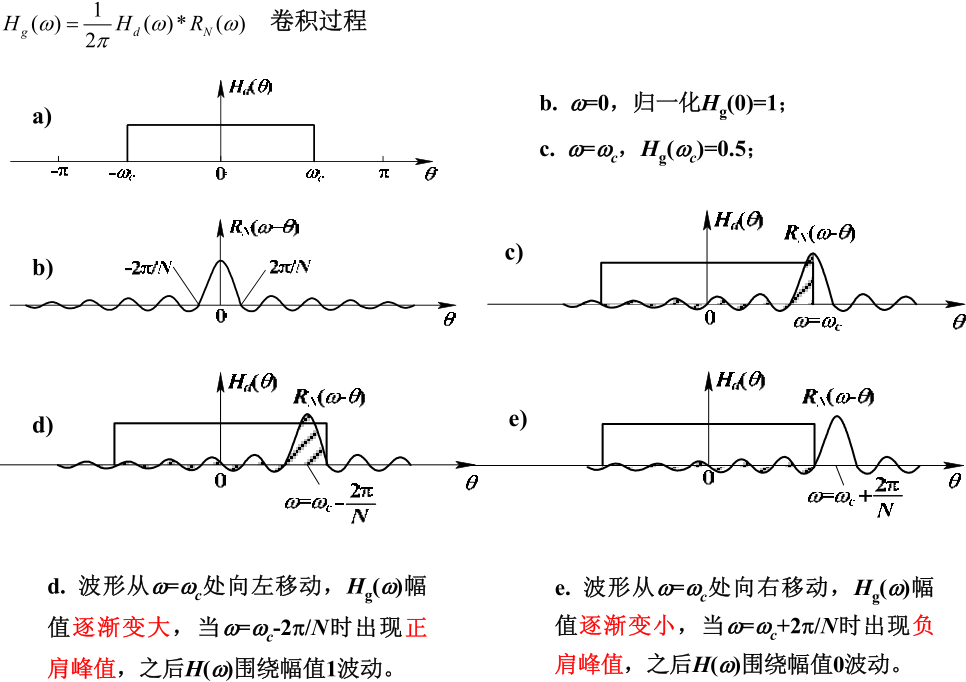
\includegraphics[width=4.5in]{fig/fig_FIR_design.png}
  \caption{FIR design process}\label{fig_FIR_design}
\end{figure}
